
\chapter{Metodologia}

{\color{red}Este capítulo dedica-se a prover uma visão geral das etapas necessárias à conclusão deste projeto, e também
permite sua eventual reprodução no futuro.}

Para a execução deste projeto, optou-se pelo uso de componentes amplamente disponíveis no mercado a relativamente baixo
custo, bem como software disponível gratuitamente no site do fabricante.


\section{Hardware}
{\color{red} Esta seção específica os componentes físicos envolvidos no robô desenvolvido para o projeto, descrevendo
também a função de cada um no desempenho das suas funções.}
{\color{red} Inserir aqui tabela com o custo dos componentes.}


\subsection{Componentes eletrônicos}

\subsubsection{Motor DC e encoder}
Para uma versão inicial do robô, foi decidido trabalhar com motor DC.
Motores DC são mais difíceis de controlar que motores de passo, porém tem uma resposta mais rápida, e se o controle for bem aplicado, podem ter um melhor desempenho que um motor de passo.
A complexidade do controle de um motor DC apresenta um bom desafio para aplicação dos conceitos e disciplinas do curso de Engenharia de Instrumental, Automação e Robôtica.
O motor DC escolhido foi um de 6V 210rpm, com taxa de redução de 1:34. O motor já possui um encoder magnético acoplado, com 11 PPR (\textit{"Pulses Per Revolution"}),
O que resulta em um encoder com resolução de 374 PPR.

\begin{figure}[htb]
	\centering
	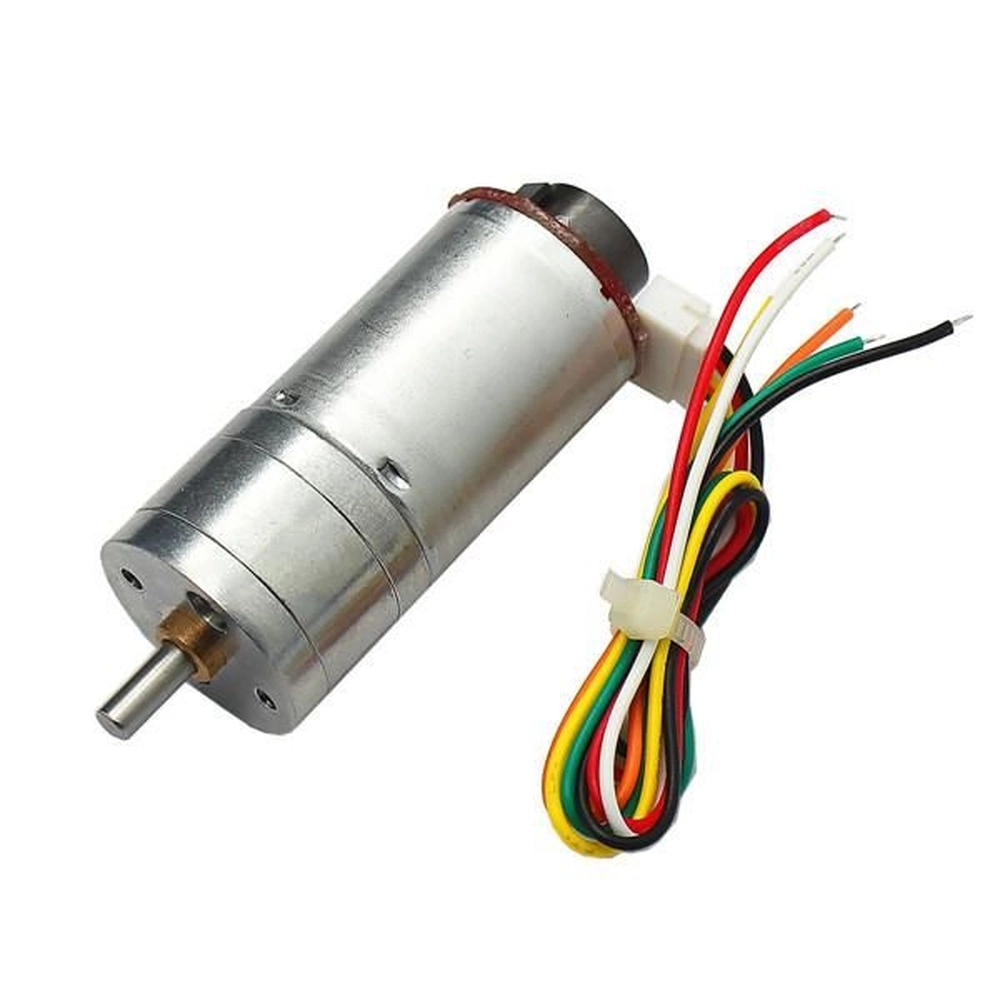
\includegraphics[width=0.7\textwidth]{figures/CHR_GM25_370}
	\caption{Motor DC 6V \cite{motor_dc_6v_encoder}}
\end{figure}

\begin{quadro}[htb]
	\caption{\label{Especificacoes_motordc_6v}Especificações do motor DC 6V}
	 \begin{tabular}{|c|c|c|c|}
		\hline
		\textbf{Componente} & \textbf{Quant} \\ \hline
		Tensão nominal & DC 6V  \\ \hline
		Velocidade sem carga  & 210RPM 0.13A  \\ \hline
		Eficiência máxima & 2,0kg.cm/170rpm/2,0W/0,60A   \\ \hline
		Poder máximo & 5,2kg.cm/110rpm/3,1W/1,10A   \\ \hline
		Torque de parada  & 10kg.cm 3.2A    \\ \hline
		Taxa de Redução do Retardador & 1:34  \\ \hline
		Resolução do salão & Razão Hall x 34,02 = 341,2PPR  \\ \hline
	\end{tabular}
	\fonte{\cite{chinhai_motor}}
\end{quadro}


\subsubsection{Driver de Motor}
Inicialmente foi testado o driver Ponte H L298N para ligar cada motor, suporta até 2A em operação DC \cite{datasheel_l298n},
a corrente de operação máxima do motor é de 1.1A, porém a corrente de parada é drenar 3.2A. 
O L298N também causa uma queda de tensão, a 1A pode causar uma queda de 3.2V, fazendo com que o
motor não receba a tensão necessária para operar nos valores desejados \cite{datasheel_l298n}. 
O L298N é mais recomendado para tensões entre 12V a 40V, como o motor é de 6v, acaba tendo uma queda de tensão considerável.
Com isso, um driver de para baixas tensões é recomendado, foi escolhido o DRV8833 \cite{datasheel_dvr8833}.


\begin{figure}[htb]
	\centering
	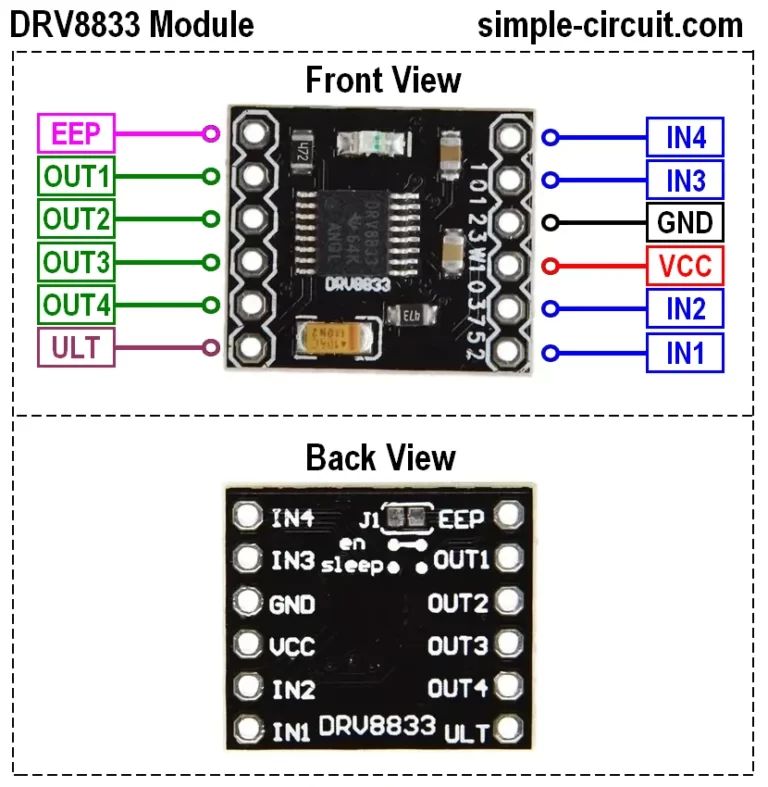
\includegraphics[width=0.5\textwidth]{figures/DRV8833-Dual-Driver-Pinout}
	\caption{Driver Ponte H DVR8833 \cite{DRV8833_image}}
\end{figure}

\subsubsection{Microcontrolador}

Para microcontrolador, optou-se pelo uso do  STM32F103C8, também conhecido como Blue Pill.
Possui como processador o ARM Cortex-M3, e tem 64Kbs de memória flash. 
O STM32F103C8 possui 7 timers, 2 ADCs, e 9 interfaces de comunicação, incluindo
I2C (\textit{Inter-Integrated Circuit}), USART (\textit{Universal Synchronous
Asynchronous Receiver Transmitter}), SPI (\textit{Serial Peripheral Interface}),
CAN e USB 2.0.
O STM32F103C8 possui 7 pinos que suportam canais de PWM de 5V, e outros 8 canais de 3.3V,  e pode ser alimentado via micro
USB de 5V. Existes 3 grupos de pinos,  $P_{A}$,  $P_{B}$ e  $P_{C}$,  os pinos PA vão de $P_{A0}$ a $P_{A15}$, PB indo de $P_{B0}$ a $P_{B15}$, e PC com apenas 3 pinos, $P_{C13}$, $P_{C14}$ e $P_{C15}$.

Para carregar o projeto no microcontrolador, um gravador ST-LINK USB será utilizado.

\begin{figure}[htb]
	\centering
	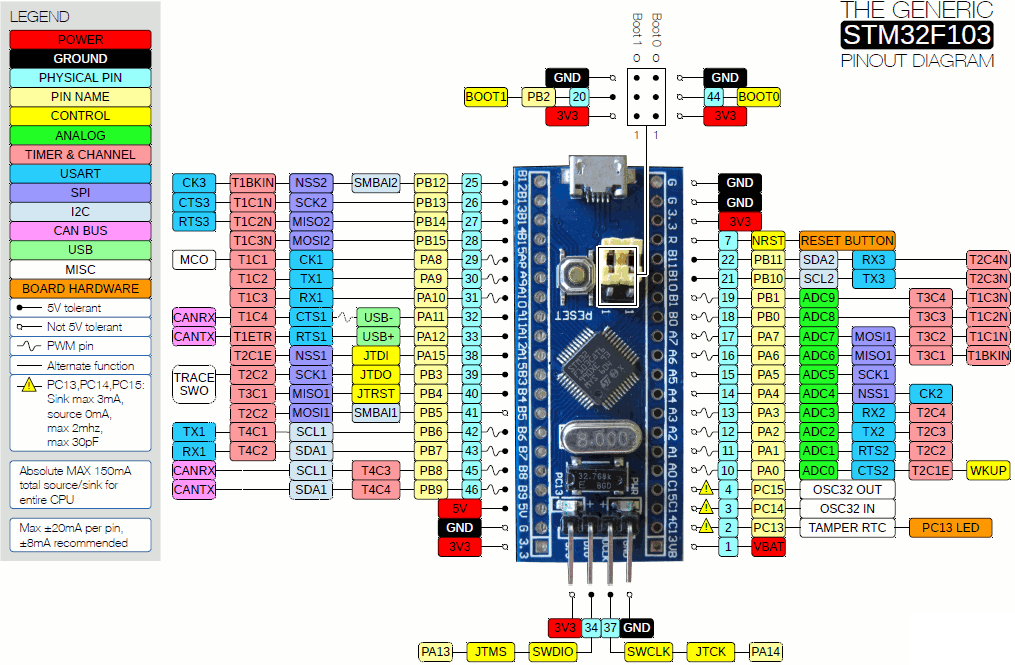
\includegraphics[width=1.0\textwidth]{figures/stm32f1_pinout}
	\caption{Diagrama de pinos do STM32F103C8}
\end{figure}

\subsubsection{Alimentação}
Para alimentar o microcontrolador, um powerbank com saída de 5v será usado, considerando que o STM32F103C8 funciona a
uma corrente abaixo de 100mA. Para alimentar os motores, para uso no desenvolvimento, optou-se por uma bateria de chumbo-ácido de 6V 4.5Ah

\subsubsection{Comunicação Bluetooth para controle em aplicativo Android - Módulo HC-5}
Para testar os movimentos do robô, decidimos usar um app android para enviar via bluetooth valores para um módulo bluetooth o HC-05, figura \ref{fig:hc_05}.
A comunicação entre o HC-05 e o stm32 será serial, usando os pinos da USART2 do stm32, o  $P_{A3}$ (RX2) e o  $P_{A2}$ (TX2).

\begin{figure}[htb]
	\centering
	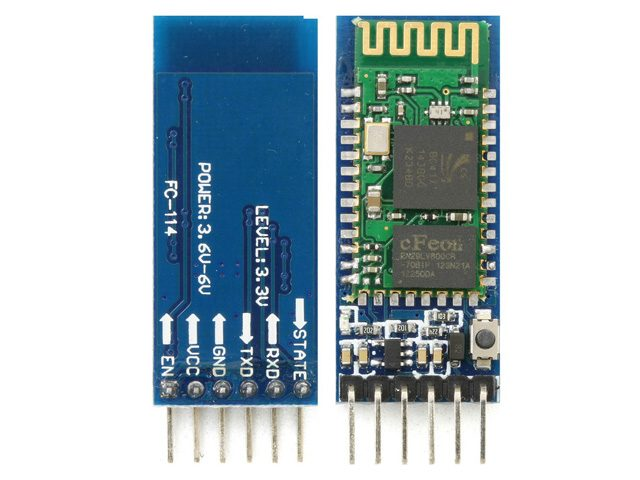
\includegraphics[width=0.5\textwidth]{figures/hc_05}
	\caption{Módulo Bluetooth HC-05}
	\label{fig:hc_05}
	\cite{hc05_image}
\end{figure}

\subsection{Componentes estruturais}

\subsubsection{Fabricação e montagem}
Foi decido fabricar o chassi e demais peças usando impressão 3D, usando filamento de PLA.
O projeto das peças foi realizado no AutoCAD e depois modelado em 3D com SolidWorks, após a modelagem realizada,
a geometria das peças foi convertida em código G para um impressora 3D usando o UltiMaker Cuda, a impressora usada foi a Ender 3 S1 Pro.


\subsection{Lista geral de componentes e materiais}

\begin{quadro}[htb]
	\caption{Lista de componentes e materias e seus custos - valores em Real (R\$)}
	 \begin{tabular}{|c|c|c|c|}
		\hline
		\textbf{Componente ou Material} & \textbf{Valor unitário} & \textbf{Quant} & \textbf{Valor Total} \\ \hline
		Driver Ponte H L298N \cite{l298n_produto} &  22,90 & 3 &  68,70   \\ \hline
		Motor DC 6V 210 RPM \cite{motor_dc_6v_produto} &  90,00 & 3 &  270,00   \\ \hline
		Filamento PLA \cite{filamento_pla_produto} &  99,99 & 1 &  99,99   \\ \hline
		Kit 4 rodas Omnidirecional \cite{omin_wheel_produto} &  131,35 & 1 &  131,35   \\ \hline
		Kit 4 peças eixo roda \cite{omin_wheel_produto} &  42,15 & 1 &  42,15   \\ \hline
		STM32 (microcontrolador) \cite{stm32_produto} &  46,90 & 1 &  46,90   \\ \hline
		Bateria selada 6V \cite{bateria_6v_produto} &  69,90 & 1 &  69,90  \\ \hline
		Powerbank &  119,90 & 1 &  119,90   \\ \hline
		Paquímetro  &  49,90 & 1 &  49,90   \\ \hline
		Ferro de solda &  43,20 & 1 &  43,20   \\ \hline
		Solda &  12,99 & 1 &  12,99   \\ \hline
		Conector mjjst macho &  4,90 & 3 &  14,70   \\ \hline
		Conector mjjst femea &  4,90 & 3 &  14,70   \\ \hline
		Garra jacaré &  1,65 & 2 &  3,30   \\ \hline
		Driver Ponte H DTV8833 \cite{drv8833_produto} &  15,00 & 3 &  45,00   \\ \hline
		Módulo Bluetooth \cite{hc05_produto} &  35,00 & 1 &  35,00   \\ \hline
		Mini Protoboard &  5,00 & 2 &  10,00   \\ \hline
		Protoboard 830 &  16,00 & 1 &  16,00   \\ \hline
		Jumper macho-macho &  8,00 & 1 &  8,00   \\ \hline
		Pasta de solda &  14,99 & 1 &  14,99   \\ \hline
		Sugador de solda &  12,99 & 1 &  12,99   \\ \hline	
		\textbf{CUSTO TOTAL} & & & \textbf{ 1.129,66}   \\ \hline
	\end{tabular}
\end{quadro}


% \subsection{Joystick de controle}
% Um joystick de 3 eixos para controlar o robô para testar a cinemática de movimento.
% {\color{red} É necessário aqui especificar o modelo utilizado e descrever características.}

% \subsection{Sensores}
% {\color{red} Esta subseção deve descrever os sensores utilizados e também sua finalidade.}

% \subsection{Dispositivos de comunicação}
% {\color{red} Esta subseção deve descrever os dispositivos de comunicação utilizados (Wi-fi, Bluetooth, etc) e também sua
% finalidade.}

% \subsection{Calibração de parâmetros}
% {\color{red} Caso haja necessidade de calibração de parâmetros de alguns dos componentes utilizados (sensibilidade de
% sensores, histerese de componentes mecânicos, taxa de comunicação de dispositivos, etc), os procedimentos devem ser
% descritos nesta subseção.}

\section{Software}
{\color{red} Esta seção se dedica a discorrer a respeito dos diversos componentes de software envolvidos no projeto.}

